%! TEX root = diss.tex
\documentclass[../diss.tex]{subfiles}
\chapter{Implementation}

% NOTE: Multiprocessor => shared memory. Use term "parallel computer" instead

% Introduction:
% * TODO: change fig 2.1 to have cloud of "graph data.csv" that interact with
%   "input graph"
% * Refer to figure 2.1, go into some more depth on interface to Parallel
%   system simulation:
%   * You create Worker implementation with access to ...., then pass
%     description to manager, specify number of workers, topology to use, num
%     computation phases, etc.
% * _Intrdc the different components, and then start going into detail in ind. subsecs_

% Some "practices used/software dev.? chapter":
% * Weekly meetings, log book,

% Graph datasets:
% * California road networks:
%   * freely-available, consisten format, real-life road network
% * Random graphs:
%   * To satisyf req. of different n
%   * Erdos-Renyi graph, but modified to be fully-connected, trick to get same properties
%     with formula for creating $p$
%   *  python library used
% * Graph reader
%   * adjacency matrix and also neighbourhood list for Dijkstra's algorithm
% * TODO: mention networkx as well as GraphReader class
% Graph datasets {{{
\section{Graph datasets}%
\label{sec:Graph datasets}

To run the algorithms, we need graphs as input. Since one important usage of \ac{APSP}
is route-planning, I used a dataset of the Californian road-network. This dataset was
initially used in \citep{graph-dataset} and has been made available on the author's
website\footnote{\url{https://www.cs.utah.edu/~lifeifei/SpatialDataset.htm}}.
% TODO: add plot of the dataset as a figure, using the python script...
This graph was used to prove that practical problems can quickly be solved on my
simulated parallel system, as long as graph compression is used.
However, for evaluation I needed graphs of various sizes, so these were generated
randomly.

\subsection{Random graph generation}%
\label{sub:Random graph generation}

% TODO: information on Erdos-Renyi graphs in prepreration chapter...

I chose to use Erd{\"o}s-Renyi graphs because they have previously been used in
evaluation of \ac{APSP} algorithms.
% TODO: cite https://core.ac.uk/download/pdf/81103122.pdf
%            https://www.researchgate.net/publication/47842024_A_Parallelization_of_Dijkstra%27s_Shortest_Path_Algorithm
I have tried to fit the parameters as closely to the real-world graph datasets
as possible. There are many characteristics of a graph, such as vertex- and
edge-connectivity, betweenness centrality, clustering coefficient, and average
distances. However, trying to generate new graphs with similar values for all
of these metrics quickly becomes a difficult problem. I have therefore only
tried to replicate the metric, \textit{average vertex degree}, which should
have some correlation to the mentioned metrics. I also want the random graphs
to be fully-connected, as most road-networks are. In the $G(n,p)$ random-graph
model, the graph is constructed by starting with a set of $n$ vertices, and
then independently include every possible edge $e$ with
% (TODO: citation???)
probability $p$. This makes the edges follow the binomial distribution:
\begin{equation}
    \textrm{deg}(v) \sim \textrm{Binomial}(n-1,p)
\end{equation}
with the average degree being $(n-1)p$. However, by instead starting with a
\textit{circular graph} and including each remaining edge independently with
probability
\begin{equation}
    p=\frac{\textrm{desired average degree} - 2}{n - 3},
\end{equation}
we get a fully-connected graph where the average degree is as desired.
% TODO: proof in appendix...
I chose the desired average degree based on the Californian road-network, which
is 2.061. However, since we will be using the compressed graph (see
\autoref{sec:Graph compression}), I used the average vertex degree of the
compressed California graph instead, which was 2.945. In
\autoref{fig:example-graph-random}, I have plotted an example graph generated
through this method. I then generated ? graphs of various sizes, from 10 nodes
to 700 nodes for use in evaluation. %TODO: how many?

\begin{table}
    \centering
    \begin{tabular}{|c|c|}
        \hline
        \textbf{Location} & \textbf{Average vertex degree} \\
        \hline
        San-Francisco (SF) &  2.549 \\
        \hline
        North-America (NA) & 2.038 \\
        \hline
        ? (OL) & 2.305 \\
        \hline
        California (cal) & 2.061 \\
        \hline
        ? (TG) & 2.614 \\
        \hline
    \end{tabular}%
    \caption[Caption]{Average vertex degree for various road-network datasets\footnotemark.}%
    \label{tab:vertex-degree}
\end{table}

\footnotetext{These values were computed using the TODO??? method in \texttt{GraphReader}.}

\begin{figure}
\begin{center}
    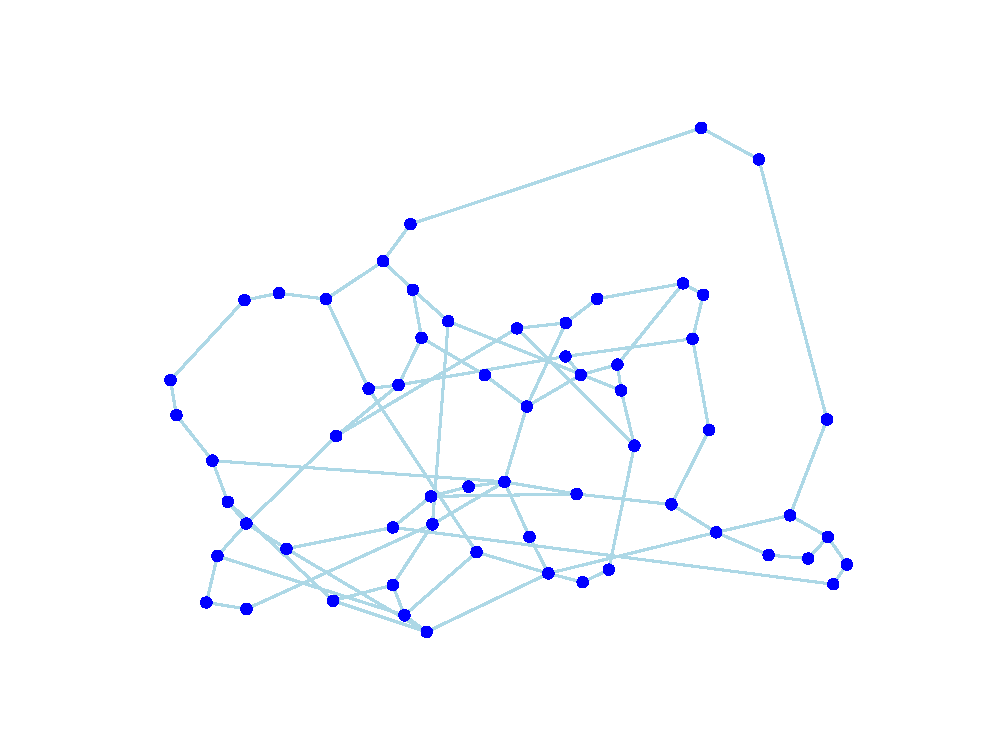
\includegraphics[scale=.7]{figs/plots/example-graph.eps}
\end{center}
\caption[Caption]{A visualisation of a graph generated with the modified
Erd{\"o}s-Renyi model. The graph has $n=60$ vertices, and the length of the
edges correspond to their weight\footnotemark[3].}%
\label{fig:example-graph-random}%
\end{figure}

\footnotetext[3]{The graph was visualised using the \texttt{ForceAtlas2} library in python. See TODO}

% \begin{algorithm}
%     \caption{Fully-connected random graph with specific average degree}%
%     \label{alg:random-graph}
%     \KwData{$n$, avg\_degree}
%     \KwResult{$G=(V,E)$}
%
%     $G \leftarrow (\textrm{set of } n \textrm{ vertices}, \emptyset)$
%
%     \For{vertices $v_{i}, v_{i+1}$}{
%         $E \leftarrow E \cup (v_{i}, v_{i+1}, w), \textrm{ where } w \sim \textrm{Uniform}[0,1]$
%     }
%     $E \leftarrow E \cup (v_{0}, v_{n-1}, w), \textrm{ where } w \sim \textrm{Uniform}[0,1]$
%
%     Not finished....
%
% \end{algorithm}


% }}}

% Simulation of a distributed memory multiprocessor:
% * Introduction:
% *   Overview of the components in bigger UML diagram, and comments on their interaction
% * Memory model (?)
%   * explain design decision behind Map : (label : String) -> (value : Number)
%   * ...
% * Timing analysis
%   * implemented as decorators for the system simulation
%   * Explain equations for how MIMD simulated (stalling bc. wait, latency+bandwidth etc.
%   * Repating computation measures, cache misses effect, possible bc.
%     seperation, mask read writes to ensure same computation done,
%     goal is more accurate eval
% Simulation of a distributed memory multiprocessor {{{
\section{Simulation of a distributed memory multiprocessor}%
\label{sec:Simulation of a distributed memory multiprocessor}

% TODO: Introduction, here we want to present the reader with the four phases and
%  the **interface** we want to create, as if reader sees diagram first, will
%  have no idea _what_ the communicationBefore, etc. is and why it's there
% * The parallel algorithms, including possible extensions, can be split into
%   3/4 phases
% * Doing this also has many benefits (TODO: go through diary and find
%   the benefits)
% * The diagram with parallel communicationBefore, then memory flush, sync barrier,
%   followed by another repeated execution, that diagram goes here and is
%   refered to

% In this "introduction 2" chapter, we explain the diagram...
\subsection{Overview of components}%
\label{sub:Overview of components}

% TODO: add comment that Manager runs whatever methods on the worker objects it has
% TODO: also add number annotations, showing how many of each they have
% TODO: shorten width of ComMan, so that can have some blue on the side
\begin{figure}[h]
\begin{center}
    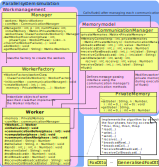
\includegraphics[scale=1]{figs/parallel-system-simulation.pdf}
\end{center}
\caption{A overview of the classes and their interaction in simulator.}
\label{fig:parallel-system-overview}
\end{figure}

In \autoref{fig:parallel-system-overview}, we see an overview of the main
components of the simulator, and how they interact. The \texttt{Manager}
constructs the specified number of \texttt{Worker}s based on some provided
subtype e.g.~\texttt{FoxOtto}, using a \texttt{WorkerFactory}. When
\texttt{doWork()} is called, it will then run the \texttt{Worker}s through all
of their communication- and computation-phases, and \texttt{flush()} the
effects of their communication after each phase, which is done using the
\texttt{CommunicationManager}. The \texttt{Worker} is an abstract class
and provides a simple yet expressive interface for algorithms ....

% Work management points:
% * Diagram of how work is simulated in parallel fashion, 8 blocks at a time
% * Use Java's executor service to avoid thread management overhead
% * Briefly remind about interace, and communication method using one object
% * Manager explain, from construction, to how doWork works, to getResult, also
%   allowing reuse of workers, which is nice ...
% * Worker factory
%   * Use of reflection, so can allow arbitrary description to be passed and
%     can still
%     crete the new worker objects that can be managed
\subsection{Work management}%
\label{sub:Work management}

When constructing the \texttt{Manager}, we specify the number of \acp{PE},
their initial memory content, and what computation they should do in each phase,
which is done by specifying the class of some implementation of
\texttt{\textit{Worker}}. When calling \texttt{doWork()} on the manager, it will
then run all the workers through a specified number of phases, where there is
3 subphases in each phase. Looking at a single worker in isolation, the execution
can be seen in \autoref{alg:execution-order}. However, these tasks are simulated
in parallel, and we must run the same subphase of all the workers before moving
onto the next because of data dependencies. This parallel execution order is
visualised in \autoref{fig:work-management-blocks}. After this is done, we can
call \texttt{getResult(label)} to extract the result by combing the
private memory of each worker into a matrix.

The worker done by each \ac{PE} is specified in subphases.  When investigating
the different algorithms, as well as possible extension like Floyd-Warshall, I
realised that they all had clear distinctions between when the \acp{PE} were
doing computation and when they were communicating. This made forcing such a
distinction in the interface not induce a reduction in flexibility. Instead of
providing an abstract method \texttt{work}, where the programmer would themself
create a \texttt{for}-loop and combine communication and computation, we
provide the four methods shown in \autoref{fig:parallel-system-overview} and
execute them as shown in \autoref{alg:execution-order}.

% TODO: can the above two paragraphs be combined somehow?

\begin{wrapfigure}{l}{0.53\textwidth}
\begin{minipage}{0.53\textwidth}
\begin{algorithm}[H]
    \caption{Execution of PE($i,j$)}%
    \label{alg:execution-order}

    $\texttt{worker.initialisation()}$\;

% \SetKwComment{Comment}{/* }{ */}
\For{$l = 0 \dots \textrm{number of phases} -1$}{
    \texttt{worker.communicationBefore($l$)}

    \texttt{worker.computation($l$)}

    \texttt{worker.communicationAfter($l$)}

}
\end{algorithm}
\end{minipage}
\end{wrapfigure}

Splitting up the work phases allows them to be represented as independent
\texttt{Callable} tasks, which has many benefits. Firstly, it allows managing
the workers using higher-level constructs like a Java \texttt{ExecutorService}
rather than using Java \texttt{Thread}. We can submit all the $p^2$ tasks in a
subphase to the executor service, and it will complete all of them without ever
spawning more than 16\footnote{This number is configurable, but since my Laptop
can execute 16 threads simultaneously, this was the optimal number} threads,
which avoids a lot of overhead. Additionally, as I will explain further in the
memory model, the side-effects of communication only happen when
\texttt{CommunicationManager::flush} is called, so there are no data
dependencies between \acp{PE} within a subphase, only between two different
subphases. Therefore I do not need locking mechanisms inside the
\texttt{\textit{Worker}}, but can instead implicitly implement them by
executing them in the order shown in \autoref{fig:work-management-blocks}.  The
third benefit is allowing repeated execution of the same work, which gives a
more accurate timing estimate.
% TODO: mention additional benefit: Easy to handle exceptions thrown by workers
%       and report them back to the caller while cleanly stopping all threads,
%       which makes development of the algortihms a lot easier, because can e.g.
%       see if receive's and send's are mismatched

% TODO: alternative diagram:
%   very small blocks with different colours, and the colours indicate whether it's
%   initilisatin, comBefore, compu, etc., and text inside is just e.g. "(0,0)"...
\begin{figure}
\begin{center}
    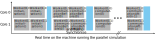
\includegraphics[scale=1]{figs/work-management-blocks.pdf}
\end{center}
\caption{Example of multithreading when simulating a 4 processing elements on
a host computer with 2 cores.}
\label{fig:work-management-blocks}
\end{figure}

The \texttt{WorkerFactory} uses Java's reflection API to create instances of
any implementation of the \texttt{\textit{Worker}} interface. When constructing
this factory, by provide a \texttt{Class} object of for instance the
\texttt{FoxOtto} implementation. It can then infer the appropriate constructor
at runtime and create $p^2$ \texttt{FoxOtto}-workers, without there being need
for a dedicated Fox-Otto worker factory. This simplifies the parallel programming
interface as implementing \texttt{\textit{Worker}} is all that is needed to
add an additional parallel algorithm to the system.

\subsection{Memory model}%
\label{sub:Memory model}

% Explains string label access
Memory is accessed through string labels. The communication
Each \ac{PE} has its own local memory, represented by a \texttt{PrivateMemory}
object. To make access as easy to use as possible for the programmer, access
is done through string labels. For example, a \ac{PE} can store some values
at location \texttt{"A"} and then retrieve it with the same label later,
additionally, for \acp{PE} handling a non $1\times 1$-sub-matrix, the
local memory is arranged in a matrix where the \ac{PE} can for instance store
values at location \texttt{(1,4,"A")} to associate it with some result related
to for example $C_{5,9}$.
% TODO: explain better above

% Communication
Introduction. To send for example data with point-to-point connections, both
the sender and recipient must call \texttt{sendData} and \texttt{receiveData},
respectively. The \texttt{receiveData(i, j, label)} method does not return a
value, but instead causes the recipient's memory at label \texttt{label} to be
set to whatever value was received. This change does not happen until
\texttt{CommunicationManager::flush()} is called, which happens in the
synchronisation phase in ?.% TODO: reference
During the flushing all the sent data is matched up with corresponding calls
to \texttt{receiveData}, and the private memories of all the recipient is
modified by the \texttt{CommunicationManager}.
An obvious alternative to this approach is making the \texttt{receiveData} method
return the actual number received, which can be done by putting the recipient
Thread to sleep until another thread has sent it data. My approach has the
following benefits and drawbacks:
\begin{itemize}
    \item[+] Separating the computation and communication gives implicit thread
        synchronisation, which allows using fewer \texttt{Thread}s, causing
        less overhead (see ) % TODO: reference manager
    \item[+] Measuring the computation time for evaluation is a lot simpler
    \item[$-$] Computation must be interleaved with a communication phase and
        we get less flexibility for algorithms where these two phases cannot
        be cleanly seperated
    \item[$-$] The \texttt{receiveData} method not returning anything is not
        an intuitive abstractions, but rather requires the programmer to know
        slightly more about the implementation of the \texttt{CommunicationManager}
\end{itemize}
% TODO: write something about how ties ties in with seperating the phases?

The main benefits are making the work management simpler, and setting up for
more accurate evaluation. The first drawback is not relevant for the algorithms
I have used. % TODO: ?

\subsection{Estimating computation and communication times}%
\label{sub:Estimating computation and communication times}

% TODO: don't know what to name a ssub here...

% The points to introduce this sub section with are:
* Diagram of how communication causes stalls, counted as comTime:
  * Split up phases into the 3 things, and can use arrow to indicate which PE
    is sending to what, and assumption on if send-before, no delay to start
    next phase...
* What is measured as computation time
* The equation for estimating communication, latency + bandwitdh * w, and
  the assumptions made behind this

We can measure the computation time directly. By taking the difference
between the CPU time before and after the computation phase, we get a measure
for how long a certain subphase took to compute, stopping the clock whenever
we enter a communication phase. We also want to minimize the
effect of running this in a simulated environment, compared to on a real
parallel system, where we would have dedicated private memory for each \ac{PE}.
% TODO: better word?
Possible effects might include the JVM suddenly performing garbage collection or
the \ac{PE}'s private memory is not in cache. To combat this, we want to repeat
each phase several times and take their average computation time.

The communication time is estimated with a theoretical model. The time it takes
to send a $s$-byte message can be modelled with $t=\alpha+\beta\cdot s$, which
is a model that has been used in other work that ... % TODO: find reference in notebook
To simplify our model, I assume that the constants $\alpha$ and $\beta$ are fixed
for all point-to-point links. Incorporating our interconnect topology, if the
shortest distance between two nodes $i$ and $j$ is $\delta(i,j)$, then the time
it takes to send a message $m$ from node $i$ to $j$ is
\begin{equation}%
\label{eq:send-time}
    t(i,j,m) \triangleq
    \delta(i,j) \cdot (\alpha + \beta \cdot \textrm{size}(m)).
\end{equation}
Since each \ac{PE} executes independently, if recipient $j$ awaits data from
sender $i$ at some time, but the sender has not reached the appropriate
communication phase by this time, the recipient must stall until $i$ is ready
and has sent the data. To model this, let $T^{(n)}_i$ be the simulated time at
which \ac{PE} $i$ starts executing phase $n$. I make the simplifying assumption
that if the recipient has received all the data it expected by the time it reaches
the corresponding communication phase, it can immediately start the next phase
after sending off the data it needs to send. With this in mind, if \ac{PE}
$i$ is receiving data from a set of sender \acp{PE} $S$ and sending data to
a set of receivers $R$ at communication phase $n$, which starts at time
$T^{(n)}_i$, then the next phase starts at
\begin{equation}%
\label{eq:communication}
    T^{(n+1)}_i = \max\left(
        \overbrace{T^{(n)}_i + \sum_{(j,m) \in R} t(i,j,m)}
        ^{\textrm{All necessary data has already arrived}}
    , \underbrace{\max_{(j,m) \in S} \left(T^{(n)}_j + t(j,i,m)\right)}
    _{\textrm{PE } i \textrm{ must stall until data has arrived}}
\right).
\end{equation}
This start time and how it is affected by late senders can be visualised in
figure % TODO: reference that figure

\subsubsection{The \texttt{timingAnalysis} package}

The functionality for measuring the computation time of each \ac{PE} and
estimating the communication time required for message-passing is implemented
using the \textit{decorator} pattern. In \autoref{fig:timing-analysis-overview},
we see an overview of the components of the \texttt{timingAnalysis} package,
where the green classes are implemented using decoration: They extend the
base class and only override methods related to timing, and use a reference to
the base object to perform the original functionality in addition to the added
timing analysis.

% TODO: blue background for what is part of the package....
% TODO: refactor Topology into this package, and include in diagram
\begin{figure}
\begin{center}
    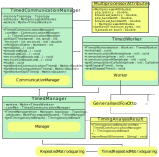
\includegraphics[scale=1]{figs/timing-analysis-overview.pdf}
\end{center}
\caption{A overview of the components of the \texttt{timingAnalysis} package.
Note that the \texttt{GeneralisedFoxOtto} and the \texttt{RepeatedMatrixSquaring}
classes are not part of this package. Additionally, the green class diagrams with
a yellow class inside it are short-hands for the decorator-pattern, where the
outer class extends the yellow inner one and contains a reference to it.}
\label{fig:timing-analysis-overview}
\end{figure}

% To explain:
% * In multiprocessorAttributes, can specify constants to use (ref equations)
% * These are used when computing message passing time in TimedComMan
% * In that class, maintain a matrix of the simulated real-time of all the \acp{PE}
%     and at each \texttt{flush()}, we update these based on stalling required
%     by the senders (as explained above...)
% * when the send or broadcast methods are called, we keep count of the number of
%   bytes sent, reset on flush, combine all in same packet possible, so programmer
%   don't need to worry about this. After this, do original functionality by
%   using held reference
% * In TimedManager, we decorate all the workers by constructing TimedWorker on them,
%   and we replace the Manager's existing \texttt{Matrix<Worker>} with these
%   using dynamic dispatch. TM also decorates the ComMan from the original Manager
% * In the TimedWorker, we use Java's \texttt{ThreadMXBean} to find the CPU time
%   each Worker spend on the CPU while running their \texttt{computation(phase :
%   int)} We also use a clever trick to minimize other effects, repeat computation
%   and take their average, not in cache, disable writes during this, so always
%   same branch, etc.

% TODO: \usepackage[nameinlink,noabbrev]{cleverref} after hyperref, and
%       use \Cref for capitals, \cref for lowercase!
The \texttt{MultiprocessorAttributes} class is used to store what constants we
assume for the message-passing latency and bandwidth, $\alpha$ and $\beta$,
both for point-to-point messages and for broadcasting. We also implement the
$\delta$ function using the \texttt{Topology} interface. Together, these two
classes are used to implement the function in \autoref{eq:send-time}, used
whenever we compute the time it takes to send a message in
\texttt{TimedCommunicationManager}.

The main timing simulation functionality happens in
\texttt{TimedCommunicationManager}. Here, we maintain a matrix of the simulated
times of each \ac{PE}, starting with $T^{(0)}_{(i,j)}$ for each of the $p^2$
\acp{PE}.  % TODO: more writing from here ....
We then update these times whenever we advance from phase $(n)$ to phase $(n+1)$,
with different rules depending on whether we have a communication phase or
a computation phase. For computation phases, we simply increment the time with
the measurement from the \texttt{TimedWorker}. For the communication phases,
we use the formula in \autoref{eq:communication}, where we build up the sets
$S$ and $R$ through decoration of the methods \texttt{sendData},
\texttt{broadcastRow}, etc. We also only evaluate this formula when executing
the decorated \texttt{flush()} method at the end of each communication phase.
We also have separate counters for how much of this simulated execution has been
used for communication, counting both time to send data and stalling until data
is ready.

\begin{wrapfigure}{l}{0.45\textwidth}
    \begin{minipage}{0.45\textwidth}
        \begin{algorithm}[H]
            \caption{Measuring computation time in \texttt{TimedWorker}}%
            \label{alg:timed-worker}
            \KwData{Phase number $l$, \textit{num.~repeats}}
            \KwResult{Computation time $t$}

            \SetKwComment{Comment}{/* }{ */}

            % \Comment*[l]{Set worker to read only}
            \tcc{Enable read-only}

            \texttt{computation($l$)}\;

            $t_0 \gets \textit{current thread CPU time }$\;

            \For{$i = 0 \dots \textrm{num. repeats} - 1$}{
                \texttt{computation($l$)}\;
            }

            $t \gets \frac{\textit{current thread CPU time } -\,t_0}{\textit{num.
            repeats}}$

            \tcc{Disable read-only}

            \texttt{computation($l$)}\;
        \end{algorithm}
    \end{minipage}
\end{wrapfigure}

In \texttt{TimedWorker}, we use a clever trick to get more accurate measures
for the computation time, as shown in \ref{alg:timed-worker}. The read-only
mode makes all side-effects of call to \texttt{Worker::store} be ignored.
This is necessary to ensure the computation always follows the same control
flow.  By running the unit of computation once before starting the timing, 
the effects of cache misses are minimized as the used data will be in cache by
the time we get to the first timed \texttt{computation($l$)}. We also do several
runs and average these to reduce the effect of short-time execution
differences on the host system.  % TODO: such as???

% Points to write in some last paragraph on why this good idea:
% * By seperating the timing functionality, we make implementation easier and
%   modularise further. When timing the program complete seperate task, so first
%   focus on simulating processor, then focus on how to time this simulation. The
%   distinction between SIMD and MIMD will also just be present here, so could
%   for instance extend further with new decorator for SIMD
% * Also follow principle of each class doing one thing, so additional functionality
%   for e.g. repeated execution not mixed with the standard worker behaivour
% * The interaction between the components above are not all explicitly redone in
%   the decorators, but are instead present from the components underneath. For
%   instance manager, just decorates all the workers the manager already have
%   created with the WorkerFactory
% * How MIMD works, the stalling time etc., explained with a diagram...

There are several benefits to separating the timing functionality from the main
functionality of the work management and memory model components, as I have
done. Firstly, it makes the program more modular, which makes implementation
easier as I could focus on fewer things at a time. It also allows the main
components to be further decorated with other timing behaviour, for example to
simulate SIMD without modifying existing code. In
\autoref{fig:timing-analysis-overview}, it looks like I am creating a whole new
layer of classes and interactions, but most of these are already implemented in
the basae components, and the interactions do not need to be reimplemented in
the decorators. % TODO: Some of this is a bit fluffy, and can probably be reduced

% Components:
% * Topology
% * MultiprocessorAttributes
% * TimedManager
% * TimedRepeatedMatrixSquaring
% * TimedWorker
% * TimingAnalysisCommunicationManager
% * TimingAnalysisResult

% }}}

% APSP via repeated matrix-squaring
% * Can abbriviate as MatSquare or something
% * Start with top-down explanation, what happens when do A^2 and same for pred. matrix
% * Then explain the driver code, why this number of iterations etc.
% * Then explain generalized fox otto algorithm, noting special case for pred. matrix
% * Explain FoxOtto (explain predecessor functionality and edge-case,
%   generalized version, pseudo-code, diagram of memory movement can go in preparation)
% * Explain driver code, and its complexity?
% * As explain, also use a simple graph as an example, going through as you do the
%   general explanation
% APSP via repeated matrix-squaring {{{
\newpage % TODO: fix this later
\section{APSP via repeated matrix-squaring}%
\label{sec:APSP via repeated matrix-squaring}

% TODO: Introduction paragraph
The \emph{\acl{MatSquare}} algorithm, which I will abbreviate as \emph{\acs{MatSquare}},
is an algorithm. \acused{MatSquare}
By using \ac{MatSquare}, we can ...

\begin{wrapfigure}{r}{0.55\textwidth}
    \begin{minipage}{0.55\textwidth}
        \vspace{-18pt}
        \begin{algorithm}[H]
            \caption{MatSquare}%
            \label{alg:matsquare}
            \SetKwInOut{Input}{Input}
            \SetKwInOut{Result}{Result}

            \Input{Adjacency matrix $W$}
            \Result{Distance matrix $M_{dist}$, Predecessor matrix $M_{pred}$}

            $M_{dist} \gets W$\;

            $M_{pred} \gets n \times n \textrm{ matrix}$\;

            \For{$(i,j) \in V^2$}{
                $M_{pred}[i,j] \gets i \textbf{ if } W_{i,j} < \infty
                \textbf{ else } j$\;
            }

            \tcp{Repeated squaring}
            \For{$x = 1 \dots \lceil \log_2 n \rceil$}{
                $M_{dist} \gets M_{dist} \otimes M_{dist}$\;
                $W \gets \textrm{witness matrix for above } \otimes$\;
                \For{$(i,j)\in V^2$}{
                    \If{$W_{i,j} \neq j$}{
                        $M_{pred}[i,j] \gets M_{pred}[W_{i,j}, j]$\;
                    }
                }
            }
        \end{algorithm}
        \vspace{-30pt}
    \end{minipage}
\end{wrapfigure}

To explain shortest paths are computed, we require two key definitions.
\begin{definition}
    A distance matrix $M_{dist}$ is a  $n \times n$ matrix, whose $(i,j)$
    entry is the length of a shortest path $i \rightsquigarrow j$ in graph
    $G=(V,E,W)$.
\end{definition}
% \begin{definition}
%     A matrix $M_{dist}^{(x)}$ is a $n \times n$ matrix where for all $0 \leq i,j<n$,
%     entry $M_{dist}^{(x)}[i,j]$ is the length of a shortest path $i
%     \rightsquigarrow j$, of at most length $x$, in graph $G$.
%     Matrix $M_{dist}^{(n)}$ is then a distance matrix.
% \end{definition}

\begin{definition}
    A predecessor matrix $M_{pred}$ is a $n \times n$ matrix, whose $(i,j)$
    entry is the immediate prior node to $j$ in a shortest path $i
    \rightsquigarrow j$.
\end{definition}

We also refer to $M_{dist}^{(x)}$ and $M_{pred}^{(x)}$ as the corresponding
matrices, but only considering paths of length \textit{at most} $x$. This then
gives that $M_{dist}^{(n)}$ and $M_{pred}^{(n)}$ are distance and predecessor
matrices, respectively\footnote{As long as the graph $G$ does not have negative
cycles}.


% TODO: keep writing here, using these four definitions..., defining W as the
%   adjecancy thing as well, and going into squaring... (also creating TODOs
%   of proofs to put in appendix...)
The goal of the \ac{MatSquare} algorithm is to compute the distance- and
predecessor matrix. If we let $W$ be the adjacency matrix for graph $G$,
and set $W_{i,i} \leftarrow 0$ for each $0 \leq i < n$, we notice that
it fits the definition of $M_{dist}^{(1)}$. Additionally, computing the
distance product between two matrices $M_{dist}^{(x)}$ and $M_{dist}^{(y)}$ gives
a matrix $M_{dist}^{(x+y)}$ containing distances shortest paths of length at most
$x+y$. As such, one way to compute the distance matrix is
\begin{equation}
    M_{dist}=M_{dist}^{(n)}=
    \underbrace{M_{dist}^{(1)} \otimes \cdots \otimes M^{(1)}_{dist}}_{n-1 \textrm{ times}}
    =
    \underbrace{W \otimes \cdots \otimes W}_{n-1 \textrm{ times}}
\end{equation}
However, we can reduce the number of distance product matrix multiplications
from $\Theta(n)$ to $\Theta(\log n)$ by squaring $W$ $\lceil \log n \rceil$
times, which is what I have done in \autoref{alg:matsquare}.

To compute the predecessor matrix, we keep track of which intermediate vertex
we use whenever we computer a distance product. When computing
$M_{i,j}=\min_{0 \leq k < n}(M_{i,k}+M_{k,j})$ as part of the distance product
$\otimes$, we refer to the used intermediate vertex as the witness for $w_{i,j}$.
\begin{definition}
    A witness matrix $W$ for a distance product $M \otimes M'$
    is a $n \times n$ matrix, where
    \begin{equation}
        w_{i,j}=\argmin_{0 \leq k < n} ( M_{i,k} + M'_{k,j})
    \end{equation}
\end{definition}
If find that $i \rightsquigarrow k \rightsquigarrow j$ is the next best path,
we use the predecessor from the path $k \rightsquigarrow j$, as long as this
path is not of length 0. This is what happens on lines 10 -- 12 in
\autoref{alg:matsquare}.

% TODO: read through all of the above, and add signposts including: "We
% implement this in driver code, and use manager to compute \otimes, distance
% product, and don't directly compute witness matrix, but same semantics....

% Define pred.matrix, distance matrix, after squaring $x$ times, why log n ceil
% squarings necessary. Explain that create Manager/Worker that implement this
% operation, so in driver code, we simply (1) prepare initial memory (2) run
% the PEs ceil times, and mem Movement such a way, no need to reset memory
% because if dist, pred in memory, assigns to "A", "B" and "P"...
% ^ could have pseuocode for this part?

\begin{wrapfigure}{r}{0.42\textwidth}
    \centering
    \fontsize{7pt}{7pt}
    \vspace{-10pt}
    \import{figs/}{fox-otto-diagram.pdf_tex}%
    \vspace{-10pt}
    \caption{Message-passing pattern used in the Fox-Otto technique.}%
    \label{fig:fox}
\end{wrapfigure}

% Introduce FoxOtto as a technique for memory movement, not a specific algo.
% Diagram of how memory moves, wrap on side to save space. Algorithm is
% in pseudocode, developed by myself with inspiration from ??? TODO: find refs
The distance product, giving our running distance- and predecessor matrices,
is computed in parallel using the parallel system simulation. We distribute
the computation across $p^2$ \acp{PE}, where each \ac{PE} executes the code
in \autoref{alg:foxOtto}. The communication is based on a technique by
\citeauthor{fox}, initially used to just perform standard matrix multiplication
\citep{fox}. Given two $n \times n$ matrices $A$ and $B$, we split them up into
$p^2$ submatrices of size $\lceil n /p \rceil \times \lceil n/p \rceil$ and
distribute them to the corresponding \acp{PE}. Before computation at each phase,
% TODO: clever ref to lower caps
we broadcast a submatrix of $A$ along each row, as shown in \autoref{fig:fox}.
After computation, we shift the $B$ submatrices upwards, wrapping around the edges.
This ensures that the corresponding entries to partially compute $C_{i,j}$
are available to \ac{PE} $(i,j)$ at each computation phase.


% Conclusion where explain time complexity and memory complexity
% and relate this to $p$, and what complexity is then...

\begin{algorithm}
    \caption{Generalised Fox-Otto execution at processing element $p_{i,j}$}%
\label{alg:foxOtto}
\SetKwInOut{Parameter}{Parameter}
\SetKwInOut{Data}{Data}
\SetKwInOut{Result}{Result}
\Data{$A_{const}',B',P'$}
\Parameter{problem size $n$, PE grid size $p$, subMatrixSize $n'=\lceil n/p\rceil$,}
\Result{$M_{dist}^{(l)},M_{pred}^{(l)}$}

\tcp{ ** Initialisation phase **}
$M_{dist}' \gets n' \times n' \textrm{ matrix}$\;
$M_{pred}' \gets n' \times n' \textrm{ matrix}$\;
\For{$0 \leq i_2,j_2 < n'$}{
    $M_{pred}'[i_2,j_2] \gets j$\;
    $M_{dist}'[i_2,j_2] \gets \infty$\;
}

\For{phase number $l = 0$ to $p-1$}{

    \tcp{ ** CommunicationBefore phase $l$ **}

    \If{$j = (i + l) \mod p$}{
        \texttt{broadcastRow(}$A_{const}'$\texttt{)}\;
    }
    \tcp{ ** Computation phase $l$ **}
    \For{$0 \leq i_2,j_2 < n'$}{
    \tcp{We start with $m$ s.t. $k=i'$ at $l=0$, which causes shorter}
    \tcp{paths from the previous squaring to be considered first.}
    \tcp{This is necessary to get the predecessor right.}
        \For{$m=i_2,i_2+1, \dots n', 0, 1, \dots, i_2-1$}{


            \tcp{In this iteration, we compute A[i', k] + B[k, j'], where}
            $k \gets (n' \cdot (i+l) + m) \mod n$\;
            $i' \gets i \cdot n' + i_2$\;
            $j' \gets j \cdot n' + j_2$\;
            \tcp{Distance product}
            $d_{new} \gets A'[i_2,m] + B'[m,j_2]$\;

            \If{$d_{new} < M_{dist}'[i_2,j_2]$}{
                $M_{dist}'[i_2,j_2] \gets d_{new}$\;
                \tcp{If $k=j'$, the path $k \rightarrow j'$ will be a self-loop, so}
                \tcp{we should not update the predecessor}
                \If{$k \neq j'$}{
                    $M_{pred}'[i_2,j_2] \gets P[m,j_2]$\;
                }
            }
        }
    }
    \tcp{ ** ComunicationAfter phase $l$ **}
    \texttt{send(}$p+i-1 \mod p$\texttt{, }$j$\texttt{, }$B'$\texttt{)}\;
    \texttt{send(}$p+i-1 \mod p$\texttt{, }$j$\texttt{, }$P'$\texttt{)}\;
}
% (subMatrixSize * (i + l) + iter) % n != 
%  subMatrixSize * j + j2
%
%  if not (j2 == iter
%      and j == (i + l) mod n)
%     update
\end{algorithm}

% Notes from reserach-and-planning diary:
% **Problem with generalized FoxOtto**:
% In the general version, we first started the multiplication by iterating from
% the top of the submatrix (see diagram in notes for $C_{10,6}$ for instance).
% However, this causes problems for the predecessor values because of the initial
% conditions. Consider the scenario for $C_{10,6}$ where want to compute path 10
% -> 10. Whenever we get to $k=10$, we would not assign predecessor because of
% exemption condition (which is necessary, otherwise we get other bugs). And at
% this point ($k=10$) we discover path of length 0. However, because of the
% generalization, we start with $k=8$ (ref. to diagram), so we find another path
% of longer length, and when we get to $k=10$, we optimize the path, but leave
% the predecessor as it was for the longer path because of the exemption
% condition. One fix is to save the initial "dist" and not use $\infty$ every
% time. Another option is making sure we start with $k=10$ when running algo i.e.
% being consistent with non-general version. That way, we immediately relax
% distance to 0 and keep the initial predecessor, this.j (or read("P") which is
% same thing). This is the option I went for, and is the reasoning behind the `m`
% loop and then modifying `iter`.
%
% * In `CountingMemoryController`, we assume
% that each PE only sends data to **one** other PE, but this is NOT CHECKED
% anywhere. However, it is enforced in underlying memory controller that each PE
% can only receive from **one** other PE, which is not equivilant, but in _most
% cases_ (all PE do the same thing) causes the above assumption to hold.

% TODO TODO: Compile list of all things about graphs, predecessors etc. that I
%            mention here, and put those in the preperation chapter!

% }}}

% Graph compression:
% * The algorithm for this, and explain all the edge cases, **with diagrams**
% * Also simple graph to use as an example
% * Also a section for the expected asymptotic speed-up referencing random graph generation
% Graph compression {{{
\section{Graph compression}%
\label{sec:Graph compression}

% Paragraph on motivation:
% * Table of number of 2-degree nodes in each graph dataset, and proportion
%   reduction, e.g. graph size reduced by 15 times
% * In general, road-networks are often very sparse
% Paragraph on how transformation works
% * Introduce notation
% * Example graph, showing how work
% Inverse transformation
% * Want to perform inverse transform as well, so extra book-keeping as compress
% * In `GraphCompressor`, which subclasses `APSPSolver`
% * Something about how nice this is, reduce computation requires, while as
%   powerful as solve the original problem as well
% Algorithm
% * Diagram of all the possible cases (look at code and `me` on how this done)
Most road networks tend to be very sparse, so many of the vertices will just
have two neighbours. We can leverage this to reduce the amount of computation
as there is only one path across a segment of two-degree nodes. We do this by
contracting all the contiguous paths of two-degree nodes into a single edge.
% TODO: clreverref
In \autoref{tab:size-reduction}, we see that this reduces the problem size by
over 16\% for all our datasets, and for some of them, like the California road
network, we have massive gains.

\begin{table}
    \centering
    \begin{tabular}{|c|c|c|c|}
        \hline
        \textbf{Road network} & \textbf{Nodes} &
        \textbf{2-degree nodes} & \textbf{Size reduction} \\
        \hline
        California          & 21048  & 19683  & $\times 15.4$ \\
        \hline
        San Francisco       & 174956 & 29627  & $\times 1.2$  \\
        \hline
        North America       & 175813 & 166687 & $\times19.3$ \\
        \hline
        City of San Joaquin & 18263  & 3760   & $\times1.26$ \\
        \hline
        City of Oldenburg   & 6105   & 3232   & $\times2.12$ \\
        \hline
    \end{tabular}%
    \caption{Possible size reduction by removing 2-degree nodes from different
    road networks}%
    \label{tab:size-reduction}
\end{table}

We compress the graph by removing all nodes with exactly two neighbours, and
the corresponding edges. We refer to a contiguous sequence of such compressed
nodes as a \textit{(compressed) chain}, and compensate for its removal by
adding a new edge between the \textit{junctions} of the compressed chain,
as shown in \autoref{fig:compression-notation}. The weight of the new edge
is the sum of the weight of the edges removed. We do this for all chains containing
at least one node of degree two. There are two edge-cases that may occur during
the compression. Firstly, if the two junctions are the same node, I set the other
junction to be one of the two-degree nodes that neighbour the junction. This is
done to not introduce further edge-cases in the path-reconstruction later.
% TODO: rename Compressed edge -> compression edge, and make colour darker
Second, if we have a two-degree-node path $p \rightarrow n_1 \rightarrow \cdots
n_l \rightarrow q$ between two junctions $p$ and $q$, and there is an edge
$(p,q) \in E$, then the compressed graph will be a have two different edges
between $p$ and $q$. In this case, we only keep the edge with the lowest
weight, discarding the other.

\begin{wrapfigure}{r}{0.36\textwidth}
    \includegraphics[scale=1]{figs/compression-notation.pdf}
    \caption{Graph before and after compression.}%
    \label{fig:compression-notation}%
    \vspace{-10pt}
\end{wrapfigure}

To get any benefit from running some \ac{APSP} algorithm, like the
\ac{MatSquare} algorithm, on the compressed graph, we must be able to map path
queries for the original graph to queries on the compressed graph, and then
map back the result. To do this, extra bookkeeping during graph compression is
needed. For each compressed node, we store a map to its two junctions, the list of
nodes in the paths to the junctions, and the length of these paths. Additionally,
with each compression edge, we store the list of compressed nodes.
To answer an \ac{APSP} query $p \rightsquigarrow q$ 
on the original graph, we visualise the graph as
shown in. % TODO: make diagram and add reference
We have 5 cases, each of which gives different queries to the original graph:
\begin{enumerate}
    \item Nodes $p$ and $q$ are on the same compressed chain, in which case
        no queries are made, and we just compute the path length from the
        bookkept information (This case is not depicted on the figure).
    \item We have $p=E,q=F$. We compute the four possible paths,
        $p \rightsquigarrow \{A,B\} \rightsquigarrow \{C,D\} \rightsquigarrow q$,
        and use the shortest one.
    \item  We have $p\in \{A,B\},q=F$. We compute the two paths, one going
        through junction $C$ and the other through $D$. The queries on the
        compressed graph are $p \rightsquigarrow C$ and $p \rightsquigarrow D$.
    \item We have $p=E,q\in \{C,D\}$. This is symmetric to case (3).
    \item We have $p\in \{A,B\}, q\in \{C,D\}$. Both nodes are on the compressed
        graph, so we query $p \rightsquigarrow q$.
\end{enumerate}
For all of the above cases, we get back a path on the form:
\begin{equation}
    p\; \rsquigarrow{nodes all in original graph}{18}\;
    J_1 \;\rsquigarrow{nodes just in compressed graph}{20}\;
    J_2 \; \rsquigarrow{nodes all in original graph}{18}\; q,
\end{equation}
where $p=J_1,J_1=J_2$, etc.~are possible. To map this back to a path in
the original graph, we must expand all the edges in the path between
the junctions, if present, $J_1 \rightsquigarrow J_2$ to a path in the original
graph. This is done by going through each edge, and swapping the compression
edges out for the list of edges that were compressed.

% }}}

% vim: foldmethod=marker
